\documentclass[runningheads,a4paper]{llncs}

\usepackage[utf8]{inputenc}
\usepackage[T1]{fontenc}
\usepackage[brazilian]{babel}
\usepackage{hyphenat}
\hyphenation{pro-ble-ma}

\usepackage{amssymb}
\usepackage{amsmath}
\usepackage{array}

\usepackage{multirow}
\newcommand{\breakcell}[2][c]{%
	\begin{tabular}[#1]{@{}c@{}}#2\end{tabular}}

%better font, similar to the default springer font
%cfr-lm is preferred over lmodern. Reasoning at http://tex.stackexchange.com/a/247543/9075
\usepackage[%
rm={oldstyle=false,proportional=true},%
sf={oldstyle=false,proportional=true},%
tt={oldstyle=false,proportional=true,variable=true},%
qt=false%
]{cfr-lm}
%
%if more space is needed, exchange cfr-lm by mathptmx
%\usepackage{mathptmx}

\usepackage{graphicx}
\graphicspath{ {images/} }

%extended enumerate, such as \begin{compactenum}
\usepackage{paralist}

%put figures inside a text
%\usepackage{picins}
%use
%\piccaptioninside
%\piccaption{...}
%\parpic[r]{\includegraphics ...}
%Text...

%Sorts the citations in the brackets
%\usepackage{cite}

%for easy quotations: \enquote{text}
\usepackage{csquotes}

%enable margin kerning
\usepackage{microtype}

%for demonstration purposes only
\usepackage[math]{blindtext}

%tweak \url{...}
\usepackage{url}
%nicer // - solution by http://tex.stackexchange.com/a/98470/9075
\makeatletter
\def\Url@twoslashes{\mathchar`\/\@ifnextchar/{\kern-.2em}{}}
\g@addto@macro\UrlSpecials{\do\/{\Url@twoslashes}}
\makeatother
\urlstyle{same}
%improve wrapping of URLs - hint by http://tex.stackexchange.com/a/10419/9075
\makeatletter
\g@addto@macro{\UrlBreaks}{\UrlOrds}
\makeatother

%diagonal lines in a table - http://tex.stackexchange.com/questions/17745/diagonal-lines-in-table-cell
%slashbox is not available in texlive (due to licensing) and also gives bad results. This, we use diagbox
%\usepackage{diagbox}

%required for pdfcomment later
\usepackage{xcolor}

% new packages BEFORE hyperref
% See also http://tex.stackexchange.com/questions/1863/which-packages-should-be-loaded-after-hyperref-instead-of-before

%enable hyperref without colors and without bookmarks
\usepackage[
%pdfauthor={},
%pdfsubject={},
%pdftitle={},
%pdfkeywords={},
bookmarks=false,
breaklinks=true,
colorlinks=true,
linkcolor=black,
citecolor=black,
urlcolor=black,
%pdfstartpage=19,
pdfpagelayout=SinglePage,
pdfstartview=Fit
]{hyperref}
%enables correct jumping to figures when referencing
\usepackage[all]{hypcap}

%enable nice comments
\usepackage{pdfcomment}
\newcommand{\commentontext}[2]{\colorbox{yellow!60}{#1}\pdfcomment[color={0.234 0.867 0.211},hoffset=-6pt,voffset=10pt,opacity=0.5]{#2}}
\newcommand{\commentatside}[1]{\pdfcomment[color={0.045 0.278 0.643},icon=Note]{#1}}

%compatibality with TODO package
\newcommand{\todo}[1]{\commentatside{#1}}

%enable \cref{...} and \Cref{...} instead of \ref: Type of reference included in the link
\usepackage[capitalise,nameinlink]{cleveref}
%Nice formats for \cref
\crefname{section}{Sect.}{Sect.}
\Crefname{section}{Section}{Sections}
\crefname{figure}{Fig.}{Fig.}
\Crefname{figure}{Figure}{Figures}

\usepackage{xspace}
%\newcommand{\eg}{e.\,g.\xspace}
%\newcommand{\ie}{i.\,e.\xspace}
\newcommand{\eg}{e.\,g.,\ }
\newcommand{\ie}{i.\,e.,\ }

%introduce \powerset - hint by http://matheplanet.com/matheplanet/nuke/html/viewtopic.php?topic=136492&post_id=997377
\DeclareFontFamily{U}{MnSymbolC}{}
\DeclareSymbolFont{MnSyC}{U}{MnSymbolC}{m}{n}
\DeclareFontShape{U}{MnSymbolC}{m}{n}{
    <-6>  MnSymbolC5
   <6-7>  MnSymbolC6
   <7-8>  MnSymbolC7
   <8-9>  MnSymbolC8
   <9-10> MnSymbolC9
  <10-12> MnSymbolC10
  <12->   MnSymbolC12%
}{}
\DeclareMathSymbol{\powerset}{\mathord}{MnSyC}{180}

\begin{document}

%Works on MiKTeX only
%hint by http://goemonx.blogspot.de/2012/01/pdflatex-ligaturen-und-copynpaste.html
%also http://tex.stackexchange.com/questions/4397/make-ligatures-in-linux-libertine-copyable-and-searchable
%This allows a copy'n'paste of the text from the paper
\input glyphtounicode.tex
\pdfgentounicode=1

\title{Aprendizado Multirrótulo Aplicado a Predição de Ocupações para Oportunidades de Trabalho}
%If Title is too long, use \titlerunning
\titlerunning{Aprendizado Multirrótulo}

%Single insitute
\author{
	Ronie Uliana e Leandro Nunes de Castro
}
%If there are too many authors, use \authorrunning
%\authorrunning{First Author et al.}
\institute{Universidade Presbiteriana Mackenzie}

%Multiple insitutes
%Currently disabled
%
\iffalse
%Multiple institutes are typeset as follows:
\author{Firstname Lastname\inst{1} \and Firstname Lastname\inst{2} }
%If there are too many authors, use \authorrunning
%\authorrunning{First Author et al.}

\institute{
Insitute 1\\
\email{...}\and
Insitute 2\\
\email{...}
}
\fi
			
\maketitle

\begin{abstract}
Esse trabalho é um estudo de caso que apresenta os resultados da aplicação de classificação multirrótulo em um problema de recrutamento de pessoas. O trabalho tenta prever quais ocupações serão atraídas para uma oportunidade de trabalho dependendo exclusivamente do título anunciado.
\end{abstract}

\keywords{multirrótulo,classificação,ensemble,contratação,recursos humanos}

\section{Introdução} \label{sec:intro}

O título anunciado em uma oportunidade de trabalho tem grande influência no tipo de pessoa que a oportunidade atrai. Um vaga com o título \enquote{Engenheiro de Custos} atrai principalmente engenheiros civis, já uma intitulada \enquote{Engenheiro Civil Júnior} tem grandes chances de atrair pessoas que atualmente são estagiários de Engenharia Civil.

Esse trabalho usa uma base de dados de mercado para tentar prever quais ocupações são atraídas pelo título da vaga. Ela acumula informação de 16 anos de uma empresa que possui um produto para o mercado de Recrutamento e Seleção e possui pouco menos de meio milhão de oportunidades de trabalho.

Os resultados mostram que é possível prever bastante bem quais são as ocupações para essas oportunidades utilizando somente o título anunciado. A intenção é incorporar o modelo gerado nesse trabalho para ajudar os recrutadores a criarem oportunidades mais assertivas.

A próxima seção define formalmente os problemas de classificação e ordenação multirrótulo, nela também é apresentada a notação usada no restante do trabalho.

As seções \ref{sec:revisao} e \ref{sec:refteo} apresentam uma breve revisão das pesquisas relevantes na área de classificação multirrótulo, com maior detalhamento nas técnicas selecionadas para o trabalho. A seguir, nas seções \ref{sec:justificativa} e \ref{sec:preparacao}, é apresentada uma justificativa para a escolha do método e  um resumo dos processos empregados para limpeza e seleção dos dados.

A seção \ref{sec:aplicacao} detalha aplicação do método, enquanto a seção \ref{sec:resultados} apresenta os resultados obtidos. Finalmente a última seção \ref{sec:conclusao} faz considerações sobre o trabalho, destacando pontos de interesse e limitações dos resultados obtidos.

\section{Definição Formal do Problema} \label{sec:formal}

Chamamos de $\mathcal{X}$ o conjunto de registros e de $\mathcal{Y}$ o conjunto com todos os rótulos possíveis. O conjunto potência $2^{\mathcal{Y}}$ é o conjunto com todos os subconjuntos possíveis de $\mathcal{Y}$.

Define-se então, formalmente, o problema de classificação multirrótulo como encontrar $h : \mathcal{X} \to 2^\mathcal{Y}$ , ou seja, encontrar a função que, dado um registro, encontra o conjunto de rótulos relacionados a ele.

Usando a mesma notação, define-se a tarefa de ordenação multirrótulo como encontrar $f : \mathcal{X} \to \mathbb{R}$ (ou $f : \mathcal{X} \to \mathbb{Z}$) a função que, dado um rótulo e um registro, retorna um valor que representa a confiança de que aquele rótulo seja correto de fato para o registro.

Para conveniência, as tabelas \ref{tab:matematica-registros}, \ref{tab:matematica-rotulos} e \ref{tab:matematica-funcoes} contêm as definições matemáticas usadas no restante do trabalho.

\begin{table}
	\centering
	\begin{tabular}{| >{\centering\arraybackslash}p{4cm} | m{8cm} |}
		\hline
		\multicolumn{2}{|c|}{\textit{Registros ou vetores de atributos}} \\
		\hline
		$\mathcal{X} = \mathbb{R}^d$ (ou $\mathcal{X} = \mathbb{Z}^d$) & $\mathcal{X}$ é o conjunto que abrange todos os registros, também pode ser entendido como o conjunto de todos os vetores de atributos (cada vetor é um registro). \\
		\hline
		$\mathcal{X} = \{\vec{x_1}, \vec{x_2}, \dots, \vec{x_n}\}$ & Mesma definição de $\mathcal{X}$ acima, mas enumerando seus elementos. \\
		\hline
		$\vec{x_i} \in \mathcal{X}$ & $\vec{x_i}$ representa um registro ou um vetor de atributos. \\
		\hline
		$d \in \mathbb{N}_{>0}$ & $d$ é o número de atributos nos registros, também pode ser compreendido como o número de dimensões nos vetores de atributos. \\
		\hline
		$\vec{x_i} = \{x_{i1}, x_{i2}, \dots, x_{id}\}$ & $\vec{x_i}$ representa um único registro do conjunto ou um vetor com $d$ atributos. No caso, $x_{ij}$ representa o valor de um único atributo. \\
		\hline
		$n = |\mathcal{X}|$ & $n$ é o número total de registros no problema. \\
		\hline
	\end{tabular}
	\caption{Notação usada para registros}
	\label{tab:matematica-registros}
\end{table}

\begin{table}
	\centering
	\begin{tabular}{| >{\centering\arraybackslash}p{4cm} | m{8cm} |}
		\hline	
		\multicolumn{2}{|c|}{\textit{Rótulos e conjuntos de rótulos}} \\
		\hline
		$\mathcal{Y} = \{y_1, y_2, \dots, y_q\}$ & $\mathcal{Y}$ é o conjunto com todos os rótulos possíveis para o problema. \\
		\hline
		$y_i \in \mathcal{Y}$ & $y_i$ representa um único rótulo. \\
		\hline
		$q = |\mathcal{Y}|$ & $q$ é o número de rótulos possíveis no problema. \\
		\hline
		$2^\mathcal{Y}$ & $2^\mathcal{Y}$ representa todos os subconjuntos possíveis de rótulos no problema (conjunto potência). \\
		\hline
		$L = {Y_1, Y_2, \dots, Y_n}$ & $L$ é a família de conjunto de rótulos, ou seja, todos os conjuntos de rótulos encontrados no problema.\\
		\hline
		$Y_i \subseteq \mathcal{Y} \wedge Y_i \in L$ & $Y_i$ é o conjunto de rótulos associado ao registro $x_i$. \\
		\hline
	\end{tabular}
	\caption{Notação usada para os rótulos}
	\label{tab:matematica-rotulos}
\end{table}

\begin{table}
	\centering
	\begin{tabular}{| >{\centering\arraybackslash}p{4cm} | m{8cm} |}
		\hline
		\multicolumn{2}{|c|}{\textit{Funções}} \\
		\hline
		$h : \mathcal{X} \to 2^\mathcal{Y}$ & $h$ é a função que mapeia os registros em subconjuntos de rótulos. Encontrar $h$ é a tarefa principal da \textbf{classificação multirrótulo}. \\
		\hline
		$f : \mathcal{X} \times \mathcal{Y} \to \mathbb{R}$ & $f$ é a função que mapeia os registros e rótulos em um número que representa a confiança que aquele é um rótulo apropriado para o registro. Encontrar $f$ é a tarefa principal da \textbf{ordenação multirrótulo}. \\
		\hline
	\end{tabular}
	\caption{Funções de classificação e ordenação}
	\label{tab:matematica-funcoes}
\end{table}	


\section{Revisão Bibliográfica}\label{sec:revisao}
Três trabalhos fornecem uma visão geral da área e fazem uma ampla revisão bibliográfica do assunto. Em \cite{Tsoumakas2007-cw}, os autores categorizam as soluções para aprendizado multirrótulo em duas:

\begin{itemize}
\item Transformação do problema;
\item Adaptação do algoritmo.
\end{itemize}

A transformação do problema consiste em torná-lo um problema de rótulo único e então usar soluções já estudadas na área. A adaptação do algoritmo altera técnicas conhecidas para classificação de rótulo único e as modifica para lidar com múltiplos rótulos.

Nesse mesmo trabalho, são enumeradas várias formas de modificação do problema e é feita uma comparação mais profunda entre três delas. São apresentados também duas métricas para caracterização dos problemas:

\begin{itemize}
\item Cardinalidade de Rótulos;
\item Densidade de Rótulos.
\end{itemize}

O trabalho da Tsoumakas e Katakis é aprimorado em \cite{Tsoumakas2009-vw}, com uma visão geral da área seguida de uma extensa revisão bibliográfica por todo o capítulo. Além da categorização anterior ele ainda divide as tarefas de aprendizado supervisionado sobre dados multirrotulados em:

\begin{itemize}
\item Classificação Multirrótulo;
\item Ordenação Multirrótulos;
\item Classificação e Ordenação Multirrótulo.
\end{itemize}

São tocados brevemente os assuntos de métricas, dimensionalidade, seleção, extração de atributos e conjuntos de dados com grande volume de rótulos. 
Mais recentemente, \cite{Zhang2014-be} revisam com mais profundidade oito dos métodos mais representativos de classificação multirrótulo e os formalizam com uma snotação matemática precisa.

\subsection{Transformação do Problema}\label{subsec:transformacao}

A transformação do problema consiste em modificá-lo para que se torne um problema de rótulo único. Dessa forma, algoritmos estudados nessa área podem ser aplicados sem alteração ao problema. Essa abordagem é primeiramente apresentada em \cite{Tsoumakas2007-cw}, recebendo apenas números como nomenclatura. Em \cite{Tsoumakas2009-vw} as transformações são expandidas com referência a novos trabalhos e recebem nomes específicos.

As abordagens mais simples citadas são por cópia e seleção. Na abordagem por cópia o os registros no conjunto de dados são repetidos uma vez para rótulo. Se um registro possui dois rótulos, ele é duplicado e cada cópia recebe apenas um dos rótulos.

Uma variação é a \emph{cópia com peso ponderado} (\textit{copy-weight}). Ela funciona como a cópia simples, mas um peso é adicionado a cada registro de acordo com o número de rótulos no registro original.

A transformação por seleção se limita e escolher apenas um rótulo em cada registro. Na variação \emph{selecionar-máximo} (\textit{select-max}), é selecionado o rótulo que mais aparece em outros registros. No \emph{selecionar-mínimo} (\textit{select-min}), o rótulo selecionado é aquele que menor frequência no conjunto de dados. A tática \emph{selecionar-aleatório} (\textit{select-random}) seleciona aleatoriamente apenas um dos rótulos do registro. Finalmente, é possível também remover todos os registros que possuam mais de um rótulo do conjunto de dados e trabalhar apenas com os que possuem um único rótulo.

A transformação \emph{Conjunto Potência} (\textit{Label Powerset}) propõe tratar um conjunto de rótulos como um rótulo único. Na sua forma mais simples, o conjunto de rótulos de cada registro se torna um novo rótulo, se o mesmo conjunto existir em outro registro, assume-se o mesmo novo rótulo.
Em conjuntos de dados que em que cada registro possui um conjunto muito distinto de rótulo, a transformação \textit{Label Powerset} acaba criando uma grande variedade de rótulos únicos, cada um com poucos registros.

A variação \emph{Random k-Labelsets} \cite{Tsoumakas2007-wm} usa um ensemble onde cada membro é treinado usando subconjuntos aleatório de rótulos como rótulos únicos.

O problema da grande quantidade de rótulos gerados pelo \textit{Label Powerset} é atacado em uma variante chamada \textit{Pruned Sets}. Essa abordagem procura reforçar as correlações mais importantes entre os rótulos, melhorando a acurácia e diminuindo a complexidade. Apesar de mais simples que o RAkEL, sua performance é ao menos equivalente \cite{Read2008-bt}.

Outra variação do \textit{Label Powerset}, chamada \textit{Ranking by Pairwise Comparison}, procura estabelecer correlações entre os rótulos dois a dois. Essa correlação é uma preferência de um rótulo sobre o outro, juntando-se todos os pares de preferências de um registro é possível criar uma ordenação dos rótulos, indo do de maior preferência até o de menor preferêcia. Elas são usadas para se criar uma ordenação multirrótulos. Cada par de rótulos possível é transformado em um único rótulo e treinado em um classificador, um algoritmo depois é responsável por unir os resultados \cite{Hullermeier2008-co}.

A ordenação da abordagem anterior é transformada em classificação multirrótulo em \cite{Furnkranz2008-rf}. O artifício usado é introduzir um rótulo virtual, sem significado, em todos os registros do conjunto de dados. O ponto onde esse rótulo virtual aparece no conjunto de rótulos predito é o ponto de corte entre os rótulos relevantes e os irrelevantes.

Uma variação do \textit{Ranking by Pairwise Comparison}, mas usando perceptrons ao invés de classificadores binários pode ser visto em \cite{Mencia2008-rh}.

A classificação por \emph{Relevância Binária} (\textit{Binary Relevance}) consiste em usar um ensemble com um classificador binário “presente/ausente” para cada rótulo. Os dois trabalhos anteriores também podem ser encarados como aplicações de Relevância Binária.

Essa abordagem tem dificuldades quando existe um grande número de rótulos diferentes, apesar do crescimento de número de classificadores necessários ser linear. Como são treinados apenas com um rótulo, também não são capazes de aproveitar as correlações entre eles na classificação. A proposta em \cite{Hullermeier2008-co} minimiza esse efeito, mas aumenta o número de classificadores necessários exponencialmente.

Essa transformação também é trabalhada em \cite{Tsoumakas2009-ex} usando uma pilha de classificadores para explorar as correlações entre os rótulos.

[TODO: Citar (UEDA; SAITO, 2002)\cite{Ueda2002-gd} com breve explicação. Propõem um método chamado Parametric Mixture Model para classificador binário]

Em (CESA-BIANCHI; GENTILE; ZANIBONI, 2006) \cite{Cesa-Bianchi2006-fk} é apresentado um algoritmo online que usa Relevância Binária em uma hierarquia de rótulos. O mesmo trabalho ainda define uma função de perda hierárquica (hierarchical loss function).

[TODO: Explicar (DEMBCZYŃSKI et al., 2012)\cite{Dembczynski2012-tv} e (TAI; LIN, 2012)\cite{Tai2012-xa} que também exploram as correlações entre rótulos para melhorar a classificação por Binary Relevance. Verificar também (ZHANG; ZHANG, 2010)\cite{Zhang2010-ee}. Relacionar também com (ESULI; FAGNI; SEBASTIANI, 2008) \cite{Esuli2008-on} que trabalha com hierarquia de rótulos, mas adaptando algoritmos]

[TODO: Verificar se vale a pena citar (CHARTE et al., 2012)\cite{Charte2012-tw} que propõe redução do número de rótulos através de regras de associação].

\subsection{Adaptação do Algoritmo}\label{subsec:adaptacao}

A adaptação do algoritmo consiste em modificar algoritmos usados em classificação de rótulo único para que trabalhem com problemas multirrótulo \cite{Tsoumakas2007-cw}.

Árvores de decisão C4.5 foram adaptadas para o multirrótulo em \cite{Clare2001-tq}. Nele, as folhas da árvore aceitam mais de um rótulo e a fórmula de entropia também foi modificada para o problema.

Duas propostas para \textit{Adaptative Boosting} com multirrótulo são feitas em \cite{Schapire2000-yt}. A primeira, \textit{AdaBoost.MH}, foi adaptada para diminuir o \textit{Hamming Loss}. Enquanto que a \textit{AdaBoost.MR} tenta encontra qual hipótese coloca os rótulos corretos no topo da ordenação.

Evoluindo esse trabalho, \cite{De_Comite2003-lg}, propõe o \textit{ADTboost.MH} que adapta o \textit{AdaBoot.MH} para possibilitar trabalhar simultaneamente com dados discretos, contínuos e textuais. As modificações nas árvores de decisão desse algoritmo também procuram facilitar a compreensão da classificação por humanos.

Em \cite{McCallum1999-iz} um classificador bayesiano para classificar os textos com multirrótulos, associando cada rótulo a uma distribuição de palavras, também facilitando a compreensão da classificação.

Nessa mesma linha de compreensão do resultado do algoritmo, \cite{Streich2008-vu} assume que os rótulos do conjunto de dados são fornecidos por fontes diferentes e mede a contribuição de cada uma na rotulação.

Uma avaliação de padrões de coocorrência de rótulos é feita em \cite{Ghamrawi2005-fw} usando \textit{Conditional Random Fields} \cite{Lafferty2001-ov}. São apresentados dois métodos: 

\begin{itemize}
\item \textit{Collective Multi-Label Classifier} traça as correlações entre pares de rótulos;
\item \textit{Collective Multi-Label with Features Classifier} correlaciona pares de rótulos a atributos.	
\end{itemize}

Ambos os métodos remetem a \cite{Hullermeier2008-co}, mas usando adaptação de algoritmo ao invés de transformação do problema.

Já o algoritmo de backpropagation é adaptado em \cite{Zhang2006-vf} com o nome de BP-MLL (\textit{BackPropagation - Multi Label Learning}).

Ainda na categoria, \cite{Crammer2003-su} propõe uma família de métodos para treinamento online baseados em perceptrons para ordenação multirrótulo.

Em \cite{Elisseeff2001-lp} é feita uma abordagem inspirada em \textit{Support Vector Machine} que tenta controlar a complexidade do classificador enquanto minimiza o Ranking Loss\todo{Ranking Loss ou Hamming Loss?}.

Ensembles de \textit{Support Vector Machines} também são utilizadas em \cite{Godbole2004-su} para classificação multirrótulo. No mesmo trabalho, as coocorrências e sobreposições de rótulos são aproveitados para melhorar os resultados.

Uma série de algoritmos baseia-se em k-vizinhos próximos. \cite{Zhang2007-id}, \cite{Luo2005-ac},\cite{Wieczorkowska2006-am}, \cite{Spyromitros2008-rs}, usam todos o mesmo algoritmo base, mas diferenciam-se na maneira como agregam os rótulos para formar o conjunto predito.
 
\textit{Multi-class, Multi-label Associative Classification} (MMAC) de \cite{Thabtah2004-vz} fornece uma alternativa na classificação multirrótulo usando regras de associação. Os rótulos são considerados de acordo com o suporte da regras.

Usando também regras de associação, \cite{Veloso2007-el} implementam uma versão lazy que aproveita os relacionamentos entre os rótulos e desempenha bem para conjuntos de dados pequenos.

\section{Referencial Teórico}\label{sec:refteo}

No aprendizado supervisionado a tarefa mais comum é encontrar um único rótulo que  caracterize um vetor de atributos (aqui chamado de \emph{registro}). O aprendizado multirrótulo também é supervisionado, porém procura encontrar o \emph{conjunto} de rótulos associado a um registro. Nesse trabalho, foi adotado o termo "aprendizado" ao invés de classificação pois essa área estuda tanto o aprendizado de funções de classificação quanto de ordenação\cite{Zhang2014-be}.

A classificação multirrótulo consiste em encontrar o conjunto de rótulos associados a um registro, já a ordenação multirrótulo se preocupa em achar uma ordem para os rótulos de acordo com a probabilidade do rótulo realmente servir para o registro, no entanto sem estabelecer um subconjunto. A classificação usando um único rótulo pode ser vista como um caso particular da classificação multirrótulo.

Existem vários problemas reais em que é natural o uso de mais de um rótulo. Por registro, na classificação de textos, uma reportagem sobre o Oriente Médio pode ser classificada como jornalismo, política ou árabe, entre outros rótulos. Uma fotografia qualquer pode ter múltiplos elementos como um barco, o mar e montanhas ao fundo e cada um desses elementos pode ser considerado um rótulo.

\marginpar{$\Leftarrow$TODO Acho que a parte em que os dados são mencionados precisa ficar em outro lugar. Está perdida aqui.}No aprendizado multirrótulo o subconjunto de rótulos possíveis aumenta exponencialmente a cada novo rótulo. No problema que esse trabalho trata, existem cerca de 8.000 rótulos diferentes, o que resulta em 28.000 subconjuntos possíveis (aproximadamente $17 \times 102.407$). Por isso, foram considerados algoritmos que exploram a coocorrência entre rótulos (Read et al. 2008), (Tsoumakas and Vlahavas 2007) e por apresentarem indícios de melhor desempenho (Tai and Lin 2012), (Zhang and Zhou 2014). 

\subsection{Classificação e Ordenação Multirrótulo}\label{subsec:classord}

A tarefa de aprendizado multirrótulo pode ser divida em dois tipos principais, dependendo da estratégia para abordá-la \cite{Tsoumakas2009-vw}. A primeira abordagem consiste em transformá-la em um problema de classificação de rótulo único, para o qual já existe extensa literatura e estudo. A segunda abordagem se apropria de algoritmos usados na classificação de rótulos únicos e os adapta para que sejam capazes de lidar com múltiplos rótulos.

\subsection{Ordens de Correlação}\label{subsec:ordcorr}

Uma das características únicas da aprendizagem multirrótulo é que, em problema reais, rótulos costumam se correlacionar. Por exemplo, uma imagem que possua o rótulo "prato" estará mais frequentemente associada com os rótulos "cozinha" ou "ingredientes" do que com rótulos como "praia" ou "areia". Estratégias que se aproveitam da correlação entre rótulos parecem ter melhor desempenho do que as que as ignoram \cite{Zhang2010-ee}.
 
É possível distinguir três tipos de estratégias quanto a correlação entre rótulos, de primeira, segunda ordem e de ordem superior.

\subsubsection{Correlação de Primeira Ordem.}

A correlação entre os rótulos não é explorada, a predição para cada rótulo é aprendida separadamente, ou seja, \emph{uma-a-uma}. O conjunto de rótulos predito para cada registro é uma união do resultado de cada aprendizado \cite{De_Carvalho2009-yp}.

\subsubsection{Correlação de Segunda Ordem.}

A correlação é explorada no formato \emph{dois-a-dois}. Cada par de rótulos é aprendido por um classificador diferente e o conjunto final é predito através da combinação entre os pares \cite{Hullermeier2008-co}.

\subsubsection{Correlação de Ordem Superior.}

Explora-se a correlação entre conjuntos maiores de rótulos \cite{Read2008-bt}, entre subconjuntos aleatórios entre si \cite{Tsoumakas2007-cw} ou com relações de hierarquia entre rótulos \cite{Vens2008-yp}, \cite{Cesa-Bianchi2006-fk}, \cite{Esuli2008-on}.

[TODO: Colocar exemplos para cada um]


\section{Transformação do Problema}\label{sec:transprob}

Existem várias estratégias que transformam um problema multirrótulo em um único problema mais simples ou em um conjunto de problemas que já possuem soluções.

O conjunto de registros na tabela \ref{tab:exbase} será usado para ilustrar as diversas estratégias de transformação.

\begin{table}
\centering
\begin{tabular}{| c | c |}
	\hline
	\textbf{Registro} & \textbf{Rótulos} \\
	\hline
	$x_1$ & $y_1$ \\
	\hline
	$x_2$ & $y_2, y_3$ \\
	\hline
	$x_3$ & $y_3$ \\
	\hline
	$x_4$ & $y_3, y_4, y_5$ \\
	\hline
	$x_5$ & $y_3, y_5$ \\
	\hline
\end{tabular}
\caption{Exemplos de registros}
\label{tab:exbase}
\end{table}

\subsection{Transformação por Cópia}

A transformação mais simples consiste em copiar os registros uma vez para cada rótulo. Usando a tabela de registros \ref{tab:exbase}, a transformação por cópia resulta na tabela \ref{tab:excopia}.

\begin{table}
	\centering
	\begin{tabular}{| c | c |}
		\hline
		\textbf{Registro} & \textbf{Rótulo} \\
		\hline
		$x_{1,1}$ & $y_1$ \\
		\hline
		$x_{2,1}$ & $y_2$ \\
		\hline
		$x_{2,2}$ & $y_3$ \\
		\hline
		$x_{3,1}$ & $y_3$ \\
		\hline
		$x_{4,1}$ & $y_3$ \\
		\hline
		$x_{4,2}$ & $y_4$ \\
		\hline
		$x_{4,3}$ & $y_5$ \\
		\hline
		$x_{5,1}$ & $y_3$ \\
		\hline
		$x_{5,2}$ & $y_5$ \\
		\hline
	\end{tabular}
	\caption{Transformação por cópia}
	\label{tab:excopia}
\end{table}

É possível observar que o número de registros cresce de acordo com o número de rótulos. Formalmente, descreve-se que cada registro $(x_i,Y_i)$ é multiplicado $|Y_i|$ vezes, substituindo $Y_i$ por $y_j \in Y_i$ em cada cópia, resultando em $(x_{ij}, y_j)$. O número de registros passa de $|\mathcal{X}|$ para $\sum_{i=1}^{n}|Y_i|$.

Essa transformação pode ser usada com um ensemble de classificadores para gerar o conjunto final de rótulos \cite{Joachims1998-zz}, \cite{Yang1999-ah}.

\subsection{Transformação por Cópia Ponderada}

Da mesma forma que a cópia do registros, mas cada rótulo recebe um valor associado que representa sua participação no registro $w = \frac{1}{|Y_i|}$.

\begin{table}
	\centering
	\begin{tabular}{| c | c | c |}
		\hline
		\textbf{Registro} & \textbf{Rótulo} & \textbf{Peso ($w$)} \\
		\hline
		$x_{1,1}$ & $y_1$ & $1$ \\
		\hline
		$x_{2,1}$ & $y_2$ & $\frac{1}{2}$ \\
		\hline
		$x_{2,2}$ & $y_3$ & $\frac{1}{2}$ \\
		\hline
		$x_{3,1}$ & $y_3$ & $1$ \\
		\hline
		$x_{4,1}$ & $y_3$ & $\frac{1}{3}$ \\
		\hline
		$x_{4,2}$ & $y_4$ & $\frac{1}{3}$ \\
		\hline
		$x_{4,3}$ & $y_5$ & $\frac{1}{3}$ \\
		\hline
		$x_{5,1}$ & $y_3$ & $\frac{1}{2}$ \\
		\hline
		$x_{5,2}$ & $y_5$ & $\frac{1}{2}$ \\
		\hline
	\end{tabular}
	\caption{Transformação por cópia}
	\label{tab:excopiapond}
\end{table}

\subsection{Transformação pela Seleção do Mínimo}

Nessa transformação, o rótulo menos frequente no conjunto $\mathcal{Y}$ é selecionado para descrever cada registro.

Formalmente:

Dado $freq : \mathcal{Y} \to \mathbb{N}_0$ como a frequência de ocorrência de um rótulo em todo o conjunto de rótulos, cada registro $(x_i, Y_i)$ é transformado em:

$$(x_i, \min_{\forall q \in Y_i} freq(q))$$

\begin{table}
	\centering
	\begin{tabular}{| c | c |}
		\hline
		\textbf{Registro} & \textbf{Rótulos} \\
		\hline
		$x_1$ & $y_1$ \\
		\hline
		$x_2$ & $y_2$ \\
		\hline
		$x_3$ & $y_3$ \\
		\hline
		$x_4$ & $y_4$ \\
		\hline
		$x_5$ & $y_5$ \\
		\hline
	\end{tabular}
	\caption{Seleção do mínimo}
	\label{tab:exselmin}
\end{table}

\subsection{Transformação pela Seleção do Máximo}

Na seleção do máximo, cada o rótulo selecionada para representar cada registro é o que ocorre com mais frequência no conjunto $\mathcal{Y}$.

Similar à seleção do mínimo, cada registro $(x_i, Y_i)$ é transformado em:

$$(x_i, \max_{\forall q \in Y_i} freq(q))$$

\begin{table}
	\centering
	\begin{tabular}{| c | c |}
		\hline
		\textbf{Registro} & \textbf{Rótulos} \\
		\hline
		$x_1$ & $y_1$ \\
		\hline
		$x_2$ & $y_2$ \\
		\hline
		$x_3$ & $y_3$ \\
		\hline
		$x_4$ & $y_4$ \\
		\hline
		$x_5$ & $y_5$ \\
		\hline
	\end{tabular}
	\caption{Seleção do máximo}
	\label{tab:exselmax}
\end{table}

\subsection{Transformação por Seleção Aleatória}

\subsection{Transformação por Ignorar Multirrótulo}

[TODO Desculpe, mas ainda não acabei de copiar o conteúdo do outro documento, Professor! Estou trabalhando nisso :p]

\section{Método Aplicado} \label{sec:justificativa}

O método escolhido para o trabalho foi o de \textit{Ensemble of Pruned Sets} \cite{Read2008-bt}.

Para esse caso, é necessário um método que tenha bons resultados e que possa trabalhar com um grande conjunto de rótulos e de registros. Vários deles se encaixam nesses requisitos, mas dois chamam especial atenção.

O método RAkEL \cite{Tsoumakas2007-wm} é referência na área, sendo um dos mais citados em trabalhos de aprendizado multirrótulo. O método usando \textit{Ensemble Pruned Sets} baseia-se no RAkEL propondo uma abordagem mais restrita e computacionalmente mais econômica.

Ambos os métodos foram considerados, mas o RAkEL foi descartado nas primeira fases da análise pelas características do problema.

O conjunto de rótulos $\mathcal{Y}$ inicial possui cerca de 485.588 rótulos distintos. A aplicação do método RAkEL \cite{Tsoumakas2007-wm} necessita de 152.227 classificadores diferentes para $k=3$, o que é bastante custoso para o caso presente.

No entanto, pela natureza do problema, é esperado que os conjuntos de rótulos possuam alta repetição. Um oportunidade de trabalho para "Enfermeiro" irá atrair frequentemente o mesmo conjunto de ocupações "enfermeiro, auxiliar de enfermagem, técnico em enfermagem", por outro lado, conjuntos muito díspares são extremamente incomuns, como "engenheiro civil, enfermeiro".

Essa intuição baseada no conhecimento do domínio foi confirmada ao se aplicar a poda de conjuntos. Apenas 268 conjuntos distintos de rótulos são responsáveis por 226.084 registros.

\section{Preparação dos dados} \label{sec:preparacao}

Como o trabalho parte de um conjunto de dados "selvagem", ou seja, não limpo nem normalizado [TODO ou seria melhor dizer "sem trabalhos prévios sobre ele"], as etapas preparatórias são de grande importância. Uma limpeza muito restritiva pode remover dados importantes, já uma muito permissiva pode deixar ruídos que dificultem a convergência de resultados.

O conjunto original possui 456.861 oportunidades de trabalho, porém nem todas possuem relevância para o trabalho. Dois são principais problemas desse conjunto.

O primeiro é que muitas oportunidades possuem uma quantidade pequena de pessoas participantes, ou mesmo nenhum. Isso ocorre em cidades pequenas, em ocupações muito especializadas, quando a redação do título possui erro ou é muito vaga. Essas oportunidades de baixa atratividade foram removidas da análise para evitar os dois últimos problemas. Isso provoca efeitos colaterais, ocupações mais especializadas não aparecem na análise e a variedade de rótulos diminui.

Foram consideradas apenas oportunidades de trabalho com mais de \textbf{50} participantes.

O segundo problema é a variedade de ocupações do participantes, não é incomum uma oportunidade com centenas pessoas possuir também centenas de ocupações distintas. Isso acontece pois não há restrição para que alguém participe de uma vaga, um pintor pode participar de uma oportunidade de arquiteto.

Apesar de comum, é pequeno o número de pessoas em uma ocupação muito divergente da oportunidade, ou seja, são poucos os pintores que participam de uma oportunidade de arquitetura. Por isso, em cada registro, foram removidas as ocupações com um número relativamente pequeno de participantes. Eventualmente, oportunidades com uma dispersão muito grande de ocupações acabam ficando sem rótulos depois que essa restrição é aplicada, registros sem rótulos como esses são removidos do treinamento.

Foram consideradas apenas ocupações que possuem mais de \textbf{5\%} de participantes dentro da oportunidade.

\begin{table}
	\centering
	\begin{tabular}{| c | c | c |}
		\hline
		& \textbf{Antes} & \textbf{Depois} \\
		\hline
		$|\mathcal{X}|$ & 377.651 & 226.084 \\
		\hline
		$|\mathcal{Y}|$ & 485.588 & 1.907 \\
		\hline
		Cardinalidade & 146,22 & 1,92 \\
		\hline
		Densidade & 0,0003 & 0,001 \\
		\hline
		Diversidade & 0,0003 & 0,001 \\
		\hline
	\end{tabular}
	\caption{Números antes e depois da preparação}
	\label{tab:preparacao}
\end{table}

Após aplicadas as restrições, os títulos da oportunidades são transformado em \textit{tokens} usando a seguinte sequência de passos.

\begin{enumerate}
	\item Remoção de palavras que contenham números ou símbolos;
	\item Remoção de \textit{stopwords};
	\item Expansão de abreviações comuns (jr, júnior; pl, pleno; sr, sênior);
	\item Remoção de acentuação;
	\item Extração do radical das palavras (\textit{stemming})
\end{enumerate}

Essa base de dados já passa por uma correção ortográfica manual no momento da publicação das oportunidades, por isso não é usado um corretor ortográfico automático na sequência de preparação.

Alguma poucas abreviações comuns específicas do domínio também são expandidas para seu nome completo.

Na etapa seguinte é aplicada a poda de conjuntos \cite{Read2008-bt}. Nela, os rótulos mais frequentes são selecionados e cada conjunto deles se torna uma classe única, transformando o problema multirrótulo em multiclasse. Esse processo resultou em \textbf{268} classes distintas para o treinamento.

\section{Aplicação do Método} \label{sec:aplicacao}

O processo de poda dos conjuntos de rótulos acontece em três fases, na primeira, encontramos os conjuntos mais frequentes de rótulos; na segunda, separamos os registros que se encaixam nesse grupo; na terceira, aplicamos uma estratégia para resgatar registros que ficaram de fora da segunda fase. O objetivo é criar o conjunto de treinamento $\mathcal{T} = \{(x_1,Y_1), (x_2, Y_2), \dots, (x_n, Y_n)\}$ a partir dos conjuntos de rótulos mais frequentes.

Seja $\mathcal{F}$ a família de conjunto de rótulos mais frequentes acima de uma certa repetição $r$:

$$
\mathcal{F} = \{Y | Y \in L; freq(L, Y) \leq r\}
$$

Onde $freq : \mathcal{Y} \times \mathcal{Y} \to \mathbb{N}$ retorna o número de vezes que $Y$ ocorre em $L$.

O conjunto de treino $\mathcal{T'}$ é formado por todos os registros onde seus rótulos são encontrados nos rótulos mais frequentes $Y \in F$. Cria-se outro conjunto $\mathcal{T''}$ através de uma estratégia de \textit{cópia} modificada para os registros que ficaram de fora de $\mathcal{T'}$. O conjunto final de treino $\mathcal{T}$ é composto pela união dos dois conjuntos anteriores.

Para formar $\mathcal{T''}$, selecionamos um registro para cada vez que um subconjunto de seus rótulos puderem ser encontrados no conjunto de frequentes $\mathcal{F}$.

\begin{align*}
\mathcal{T'} &= \{(\vec{x_i}, Y_i) | Y_i \in \mathcal{F}\} \\
\mathcal{T''} &=  \{(\vec{x_i}, Y') | (\vec{x_i}, Y_i) \notin \mathcal{T'}; Y' \in \mathcal{F}; Y' \subset Y_i \} \\
\mathcal{T} &=  \mathcal{T'} \cup \mathcal{T''}
\end{align*}

Depois de criado o novo conjunto de treino $\mathcal{T}$ transforma-se cada conjunto de rótulos encontrado em $\mathcal{F}$ em um rótulo único. A partir desse ponto, o problema se transforma em um problema de classificação multiclasse.

É usado então um \textit{ensemble} de classificadores binários\footnote{Foram usados classificadores SVM (Support Vector Machine)} para selecionar quais rótulos fazem parte da resposta. A maneira como é montado o conjunto resultado é diferente do proposto originalmente no modelo de \textit{Pruned Sets} \cite{Read2008-bt}. Nele, apenas o classificador com melhor resultado retorna sua predição\footnote{Esse modelo é conhecido como \textit{one-vs-rest} \cite{Bishop2006-vm}}, nesse, cada classificador com retorno positivo soma seus rótulos associados a um multiconjunto (\textit{bag} ou \textit{multiset}) que será retornado como resposta da classificação. Posteriormente, um limite de corte é estabelecido para eliminar rótulos menos votados.

Em testes preliminares, essa modificação apresentou melhores resultados, permitindo que o modelo gerasse como resposta conjuntos de rótulos que não estavam no conjunto de treino.

Digamos, por exemplo, que possuímos apenas dois classificadores, um associado ao conjunto de rótulos $\{magro, alto\}$ e outro associado a $\{magro, baixo\}$. Se ao passar por ambos os classificadores o registro tiver retorno positivo apenas no primeiro, a resposta resultante será $\{(magro, 1), (alto, 1)\}$. Se os dois classificadores retornarem positivo, a resposta final seria $\{(magro, 2), (alto, 1), (baixo, 1)\}$.

Uma função $t$ é usada para restringir o conjunto resposta aos rótulos mais relevantes. No exemplo anterior, se $t$ considerar apenas rótulos que 2 ou mais classificadores concordem, o conjunto resultante passa a ser apenas $\{magro\}$.

Para ampliar esse efeito, o modelo é replicado 10 vezes para se criar um novo \textit{ensemble}. Cada um é treinado por $2/3$ dos dados e o mesmo método para geração dos conjuntos resposta é aplicado para o \textit{ensemble} como um todo.

\section{Resultados} \label{sec:resultados}

O modelo foi feito utilizando-se porções menores do conjunto total de dados para que o desenvolvimento pudesse ser feito em ciclos rápidos. Foram usadas massas aleatórias com 1\%, 5\% e 10\% do total.

Após o desenvolvimento do modelo, toda a massa de dados é usada para treinamento e validação. A validação do modelo é feita usando-se a técnica de \textit{cross-validation} \cite{Kohavi95-as} usando o conjunto dividido em \textbf{5} partes.

Os resultados são avaliados por métricas que possuem sentido para o domínio, no caso, prever ocupações atraídas para uma oportunidade de trabalho. A primeira métrica é a precisão, nesse contexto ela responde a pergunta "quantas ocupações foram preditas corretamente?". Outra métrica relevante é a revocação (\textit{recall}), no domínio proposto ela responde a pergunta "quantas ocupações deixaram de ser preditas?". Finalmente, o \textit{F1 Score} é uma medida geral de quão bem as duas perguntas anteriores são respondidas.

Em problemas multirrótulo cada registro do conjunto de teste tem suas próprias métricas, para obter uma visão geral de quão bem o modelo se comporta basta calcular as medidas centrais de toda a amostra.

\begin{align*}
Precisão_i(h) &= \frac{|Y_i \cap h(x_i)|}{|h(x_i)|} \\
Revocação_i(h) &= \frac{|Y_i \cap h(x_i)|}{|Y_i|} \\
F1_i(h) &= 2 \cdot \frac{Precisão_i(h) \cdot Revocação_i(h)}{Precisão_i(h) + Revocação_i(h)} 
\end{align*}

Como a distribuição do resultado não é regular, são utilizados o 1º, 2º e 3º quartis como medidas de adequação.

\begin{table}
	\centering
	\begin{tabular}{| c | c | c | c |}
		\hline
		& & \breakcell{1 Classificador\\Limite 2} & \breakcell{10 Classificadores\\Limite 18} \\
		\hline
		\multirow{3}{*}{Precisão} & 1º Quartil & 0,33 & 0,50 \\
		& 2º Quartil & 0,50 & 1,00 \\
		& 3º Quartil & 1,00 & 1,00 \\
		\hline
		\multirow{3}{*}{Revocação} & 1º Quartil & 0,50 & 0,50 \\
		& 2º Quartil & 1,00 & 1,00 \\
		& 3º Quartil & 1,00 & 1,00 \\
		\hline
		\multirow{3}{*}{F1 Score} & 1º Quartil & 0,50 & 0,50 \\
		& 2º Quartil & 0,67 & 0,67 \\
		& 3º Quartil & 0,80 & 1,00 \\
		\hline
	\end{tabular}
	\caption{Resultados com 1 e 10 classificadores e os melhores limites}
	\label{tab:resultado}
\end{table}

É possível observar na tabela \ref{tab:resultado} que a utilização de 10 classificadores melhora a precisão significativamente, mas possui pouco efeito na revocação e no \textit{F1 Score}. O tempo de treinamento para os 10 classificadores é obviamente 10 vezes maior do que o de um único classificador, apesar disso, como o treinamento nesse domínio será feito anualmente, o ganho em precisão paga o tempo extra.

Outro ponto de atenção é que a distribuição dos resultados não segue a curva normal, como é possível observar na figura \ref{fig:medicoes}, a maior parte do conjunto de teste se concentra nas pontuações mais altas das medições.

\begin{figure}
	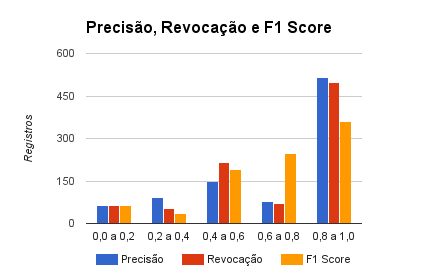
\includegraphics[scale=0.7]{medicoes}
	\caption{Distribuição das medições}
	\label{fig:medicoes}
\end{figure}


\section{Conclusão} \label{sec:conclusao}

[TODO]
\begin{itemize}
	\item Passar a definição formal do problema como segunda seção!
	\item Rodar cross-validation com todos os dados, atualizar a tabela e refazer os gráfico. É improvável um resultado muito diferente, então (espero) que eu não tenha que modificar o texto.
	\item Melhorar os gráficos. Achei que ficaram muito feios =/
	\item Observação: os resultados são intuitivamente muito bons mesmo quando a precisão não parece boa. Isso ainda precisa ser confirmado.
\end{itemize}

%%%%%%%%%%%%%%%%%%%%%%%%%%%%%%%%%%%%%%%%%%%%%%%%%%%%%%%%%%%%%%%%%%%%%%%%%%%%%%%
\bibliographystyle{splncs03}
\bibliography{paper}
%%%%%%%%%%%%%%%%%%%%%%%%%%%%%%%%%%%%%%%%%%%%%%%%%%%%%%%%%%%%%%%%%%%%%%%%%%%%%%%

\end{document}
